\documentclass[12pt]{article}
\newcommand{\bottomMargin}{2cm}


\newcommand{\header}{
	ДИЗАЙН И АНАЛИЗ НА АЛГОРИТМИ - \\ ПРАКТИКУМ\\
	\vspace{0.1cm}
        Летен семестър, 2026 г., първо контролно\\
	\vspace{0.1cm}
}
\newcommand{\tl}{$1.2$ сек.}
\newcommand{\ml}{$256$ MB}

\input{structure.tex}

\begin{document}

\section{Задача К1. Вази}

\begin{wrapfigure}{r}{0.30\textwidth}
	\begin{adjustbox}{width=0.30\textwidth}
		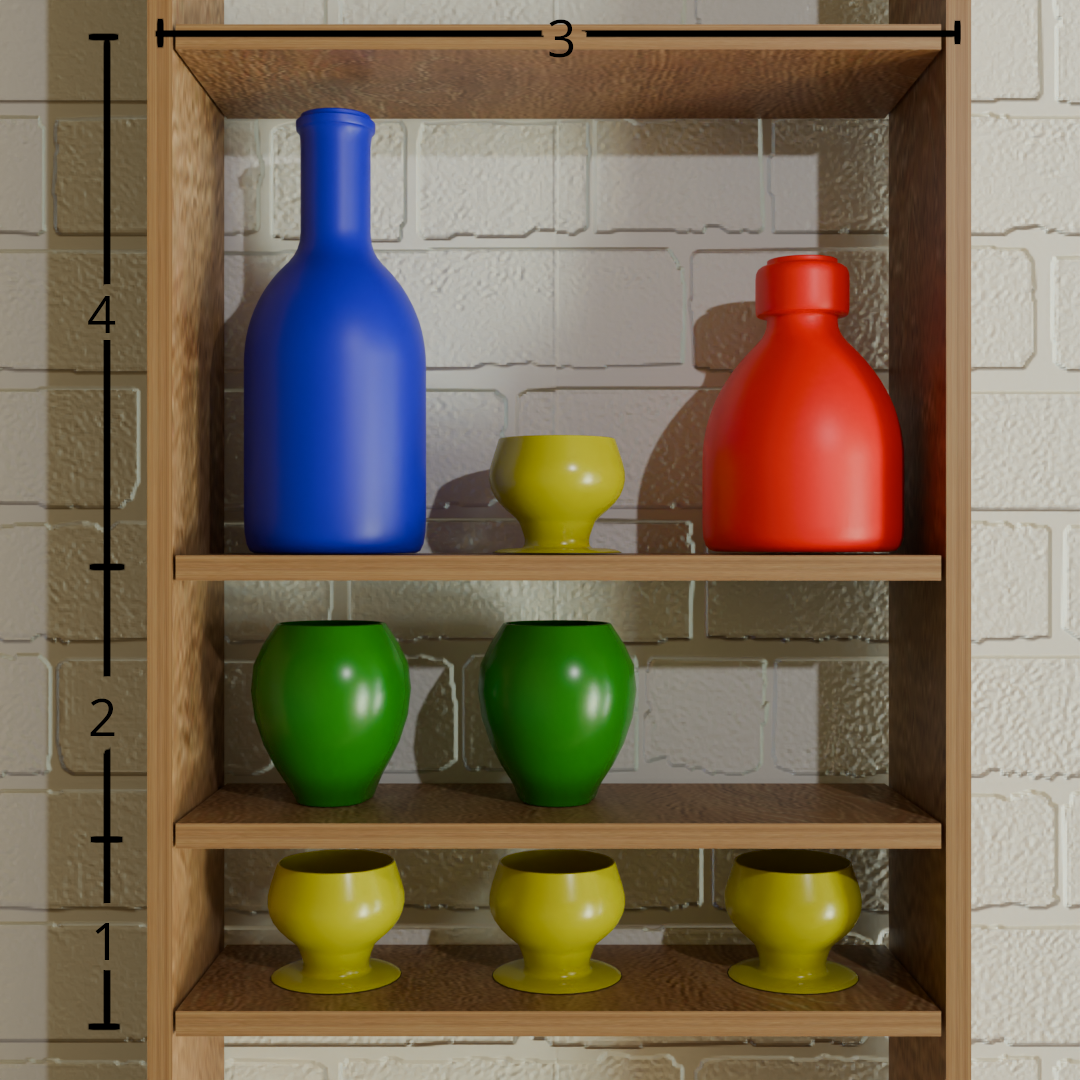
\includegraphics{vazi_lab.png}
	\end{adjustbox}
\end{wrapfigure}

Боби Вазимиров е прочут грънчар. Напоследък получил толкова вдъхновение и изработил толкова много вази, че вече няма къде да ги съхранява. Затова решил да изгради шкаф с рафтове върху една от стените в работилницата си.

Той разполага с $N$ вази с височини $A_1, A_2, \dots, A_N$. Всички вази имат еднакъв диаметър (широчина) $1$.

Стената, върху която ще бъде поставен шкафът, е с обща височина $H$. Боби може да поставя произволен брой хоризонтални рафтове. Всеки рафт заема цялата широчина на шкафа (от единия край до другия). Рафтовете могат да бъдат разположени на произволни височини, което означава, че разстоянията между съседни рафтове (височините на отделните отделения) могат да са различни. Сумата от височините на всички отделения не трябва да надвишава $H$. Може да се счита, че рафтовете са с пренебрежимо малка дебелина.

Една ваза може да бъде поставена в дадено отделение само ако височината на това отделение е по-голяма или равна на височината на вазата. В едно отделение могат да се поставят няколко вази една до друга.

Боби иска шкафът да заема възможно най-малка широчина, но е твърде зает с правенето на вази, и затова Ви моли за помощ. Намерете минималната широчина на шкаф, в който могат да се поберат всички вази.

Напишете програма \textbf{vases}, която да намира търсената минимална възможна широчина на шкафа.

\subsection{Вход}
От първия ред на стандартния вход се въвеждат $2$ цели естествени числа $N$ и $H$ -- съответно броят на вазите и височината на стената. На втория ред се въвеждат $N$ числа -- $A_1, A_2, \dots, A_N$ -- височините на вазите.

\subsection{Изход}
На единствения ред на стандартния изход изведете едно цяло число -- търсената минимална ширина на шкафа. 

\subsection{Ограничения}
\vspace{0.1em}
\begin{itemize}
	\item $1 \leq N \leq 10^7$
	\item $1 \leq H\leq 10^7$
    \item $1 \leq A_i \leq H$
\end{itemize}

\subsection{Подзадачи}
\begin{table}[H]
	\begin{tblr}{|Q[c,m]|Q[c,m]|Q[c,m]|Q[c,m]|X[c,m]|}
		\hline
		\textbf{Подзадача} & \textbf{Точки} & \textbf{Необходими подзадачи} & $N$ & \textbf{Други ограничения}\\
		\hline
		$0$ & $0$ & $-$ & $-$ & Първият примерен тест. \\ 
		\hline
		$1$ & $7$ & $-$ & $\leq 10^3$ & Всички стойности на $A_i$ са равни. \\ 
		\hline
		$2$ & $14$ & $-$ & $\leq 10^3$ & Има точно две различни стойности на $A_i$. \\ 
		\hline
		$3$ & $15$ & $0-2$ & $\leq 10^3$ & $-$ \\ 
		\hline
		$4$ & $35$ & $0-3$ & $\leq 10^5$ & $-$ \\
		\hline 
		$5$ & $29$ & $0-4$ & $\leq 10^7$ & $-$ \\
		\hline
	\end{tblr}
	\caption*{Точките за дадена подзадача се получават само ако се преминат успешно всички тестове, предвидени за нея или за някоя от необходимите подзадачи.}
\end{table}
\FloatBarrier

\subsection{Пример}
\begin{table}[H]
	\begin{tblr}{|l|l|X[j]|}
		\hline
		\textbf{Вход} & \textbf{Изход} & \textbf{Обяснение на примера} \\
		\hline
		\texttt{\makecell[lt]{8 7\\
		2 1 1 3 2 4 1 1    
		}}
		& 
		\texttt{\makecell[lt]{3}}
		& 
		{Вижте картинката. \\ Жълтите вази са с височина $1$, зелените с височина $2$, червената е с височина $3$, а синята -- с $4$.}\\
		\hline
		\texttt{\makecell[lt]{5 5\\
		1 1 1 1 1  
		}}
		& 
		\texttt{\makecell[lt]{1}}
		& 
		\\
		\hline
	\end{tblr}
\end{table}
\FloatBarrier

\end{document}
